%
% File acl2020.tex
%
%% Based on the style files for ACL 2020, which were
%% Based on the style files for ACL 2018, NAACL 2018/19, which were
%% Based on the style files for ACL-2015, with some improvements
%%  taken from the NAACL-2016 style
%% Based on the style files for ACL-2014, which were, in turn,
%% based on ACL-2013, ACL-2012, ACL-2011, ACL-2010, ACL-IJCNLP-2009,
%% EACL-2009, IJCNLP-2008...
%% Based on the style files for EACL 2006 by 
%%e.agirre@ehu.es or Sergi.Balari@uab.es
%% and that of ACL 08 by Joakim Nivre and Noah Smith

\documentclass[11pt,a4paper]{article}
\usepackage[hyperref]{acl2020}
\usepackage{times}
\usepackage{latexsym}
\usepackage{graphicx}
\renewcommand{\UrlFont}{\ttfamily\small}

% This is not strictly necessary, and may be commented out,
% but it will improve the layout of the manuscript,
% and will typically save some space.
\usepackage{microtype}

\aclfinalcopy % Uncomment this line for the final submission
%\def\aclpaperid{***} %  Enter the acl Paper ID here

%\setlength\titlebox{5cm}
% You can expand the titlebox if you need extra space
% to show all the authors. Please do not make the titlebox
% smaller than 5cm (the original size); we will check this
% in the camera-ready version and ask you to change it back.

\newcommand\BibTeX{B\textsc{ib}\TeX}

\title{The Dark Side of Language: Using NLP to Combat Hate Speech}

\author{ 
  Adam Hyman, 
  %\texttt{adamhyman@berkeley.edu} \\
  Shalini Chawla,
  %\texttt{schawla@berkeley.edu} \\
  Sreeram Ravinoothala \\
  %\texttt{sreeram@berkeley.edu} 
  }

\date{April 2023}

\begin{document}
\maketitle
\begin{abstract}
With the advent of social media, people have had access to propagate hate anonymously, making it more dangerous than ever as the impact is not contained by a social group or geographic area. It is very important for social media companies to accurately identify hateful content and remove it as the impact can be far fetched. In addition to just flag hateful content with a binary label, it is useful to identify the hate category, which can be further used to study any correlations between social-political events and its impact on specific categories of hateful content in online media. In this paper, we fine-tune three pre-trained large language models for a multi-label classification task to categorize user comments as toxic, severe\_toxic, obscene, threat, insult and identity\_hate. To help our models with accurately identifying the minority classes, we explore back translation as an option to augment existing data.

\end{abstract}

\section{Introduction}

In common language, “hate speech” refers to offensive discourse targeting a group or an individual based on inherent characteristics (such as race, religion or gender).

The adoption of Social media brings in different views of many people. One of the primary issues bleeding the social media community is hate speech. Hate speech brings lot of negativity in people that if not curtailed can spiral into bigger issues like what we see around us in many cases. Hate speech can be targeted against individual, community, ideology etc. The social platforms with so many resources at hand are able to take care of it though much more is needed to cut it at the root.

With the advances in AI/ML, many of the social media platforms have done a lot of great work in controlling the proliferation of hate speech by making use of classification algorithms but there is much more to be done to reduce the exposure to a great extent.

Hate speech on social media platform is well known and the platforms are employing different techniques to bring the exposure down. They are successful in many ways but classifying the content to check if it indeed is hate is very complex as it depends on the context as well as whether its used loosely. There is lot of research done or going on classifying the text as well as augmenting such text.

The ability in building accurate models to correctly classify hateful content is a challenging task due to the limited availability of labeled data required for training. The training data needs to be labeled by human annotators. In addition to being a tedious task, it also exposes the annotators to the disturbing content in the data they are required to label. The public data sets available today are highly imbalanced and have very limited samples for some of the minority categories including threat, obscene and severe\_toxic compared to the large amount of non-toxic samples. We follow two approaches to deal with the limitations of data availability.

1) We use pre-trained large language models and fine tune them for a classification tasks. Using a pre-trained model gives us the ability to use smaller amount of training data to achieve the same performance that would have required a much larger training data set with a classifier built from ground up.

2) We use data augmentation to further balance our data set across the toxic classification categories. We have three minority categories: threat, severe-toxic and identity\_hate that have very low representation in our training data set. We use the TOXIGEN data set to augment data for the identity\_hate class. To augment data for the other classes, we use reverse translation to generate additional samples from the existing data. 



\section{Background}
The task of toxic content classification has been tackled before using many different approaches. The availability of quality labeled data has been widely accepted as a limitation in the ability to create accurate models for toxic content classification.
(Rastogi et al.) has explored generating synthetic data using EDA and back translation to augment the training data and reported improved recall and F1 scores. (Hartvigsen et al., ACL 2022) have used GPT-2 to generate synthetic identity_hate data to help improve the claasification accuracy of implicit conent. 


\section{Data}

\subsection{Source Data Set}
We use the jigaw dataset from kaggle competition that was derived out of reddit data. The data set consist of 3 files that includes the labeled training data, test data and the test labels. We combine the test data and labels file by joining them on the unique comment identifiers. The training data set has 159,000 samples while the test data set has 60,000 samples. We convert the comments into lowercase and clean the contents by removing punctuation and special characters. Once processed both are training and test data file  consist of the text comments and binary labels for the 6 categories listed below.

\begin{itemize}
\item toxic
\item severe\_toxic
\item obscene
\item threat
\item insult
\item identity\_hate
\end{itemize}

\subsection{Data Balancing}
Our source data is highly imbalanced. Out of the 6 labeled classes, 3 are majority classes with and 3 are minority classes.
\begin{table}
\centering
\begin{tabular}{l r}
\hline
\textbf{Label} & \textbf{Count}\\
\hline
\verb|toxic| & 159000 \\
\verb|severe_toxic| & 1500 \\
\verb|obscene| & 500 \\ 
\verb|threat| & 500 \\ 
\verb|insult| & 500 \\
\verb|identity_hate| & 500 \\
\hline 
\end{tabular}
\caption{Distribution of toxicity labels in the source data set.}
\end{table}

\begin{figure}[h]
\centering
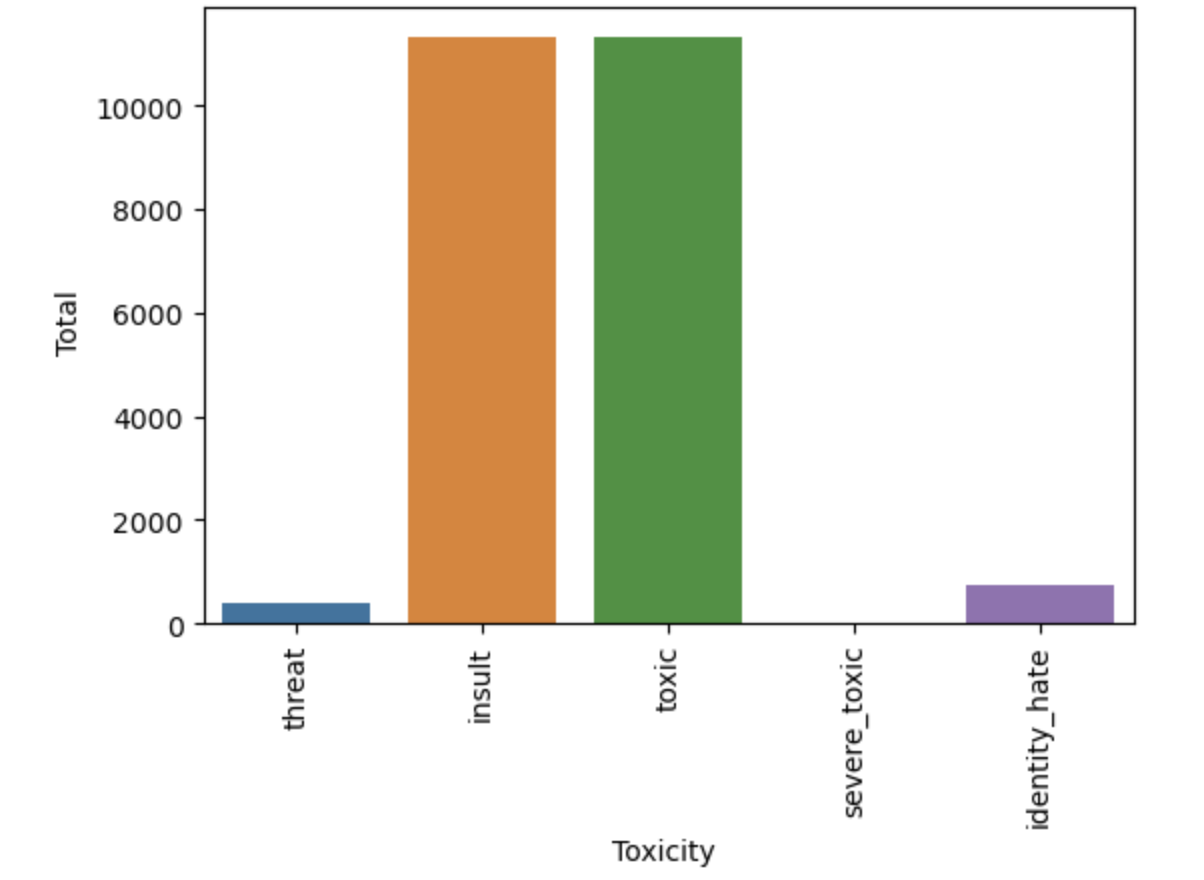
\includegraphics[scale=0.4]{label_counts.png}
\caption{Toxicity Label Count}
\end{figure}

\subsection{Undersampling Majority Class Data}
To balance the data set for the 6 classes being identified, we use a combination of strategies. We undersample two of two majority classes severe\_toxic and obscene to select 2000 random samples each from the original training data set. Since the label toxic is set to True if any of the 

\subsection{Augmenting Minority Class Data}
To bring the available training data for minority classes to be closer in count to the majority classes more balanced To augment the data for minority classes identity\_hate, we chose to augment with the data available from the TOXIGEN dataset[2]


\section{Methods}

\subsection{Baseline Model}
Our baseline model is BERT base model(cased). We fine-tune the model on the full training data set that has been split into training and validation using 80:20 split and stratified on the 6 label classes. We add a hidden layer with 200 neurons and dropout layer with 0.3 before our final classification layer with 6 outputs to perform a multi label classification. We train the model for 2 epochs using learning rate of .00005 and batch size of 32.

As expected, the model performs really poorly for our 3 minority classes.

\begin{table}
\centering
\begin{tabular}{lrrr}
\hline
\textbf{class} & \textbf{prec} & \textbf{recall} & \textbf{f1-score}\\
\hline
\verb|toxic| & 0.62 & 0.40 & 0.49 \\
\verb|severe_toxic| & \textcolor{red}{0.00} & \textcolor{red}{0.00} & \textcolor{red}{0.00} \\
\verb|obscene| & 0.66 & 0.32 & 0.43 \\
\verb|threat| & \textcolor{red}{0.00} & \textcolor{red}{0.00} & \textcolor{red}{0.00} \\
\verb|insult| & 0.65 & 0.25 & 0.36 \\
\verb|identity_hate| & \textcolor{red}{0.00} & \textcolor{red}{0.00} & \textcolor{red}{0.00} \\
\vspace{2\baselineskip}\\
\verb|micro avg| & 0.64 & 0.31 & 0.42 \\
\verb|macro avg| & 0.32 & 0.16 & 0.21 \\
\verb|weighted avf| & 0.58 & 0.31 & 0.40 \\
\verb|samples avg| & 0.04 & 0.03 & 0.03 \\
\hline
\end{tabular}
\caption{Baseline Model - Classification Report}
\end{table}


\subsection{T5}

\subsection{ELECTRA}

\section{Results and Discussion}

\section{Error Analysis}

\section{Conclusion}

\section*{References}
Rastogi, Chetanya, et al. “Can We Achieve More with Less? Exploring Data Augmentation for Toxic Comment Classification.” ArXiv:2007.00875 [Cs], 2 July 2020, arxiv.org/abs/2007.00875. Accessed 31 Mar. 2023.\\\\
Thomas Hartvigsen, Saadia Gabriel, Hamid Palangi, Maarten Sap, Dipankar Ray, and Ece Kamar. 2022. ToxiGen: A Large-Scale Machine-Generated Dataset for Adversarial and Implicit Hate Speech Detection. In Proceedings of the 60th Annual Meeting of the Association for Computational Linguistics (Volume 1: Long Papers), pages 3309–3326, Dublin, Ireland. Association for Computational Linguistics.



\label{sec:length}

The conference accepts submissions of long papers and short papers.
Long papers may consist of up to eight (8) pages of content plus unlimited pages for references.
Upon acceptance, final versions of long papers will be given one additional page -- up to nine (9) pages of content plus unlimited pages for references -- so that reviewers' comments can be taken into account.
Short papers may consist of up to four (4) pages of content, plus unlimited pages for references.
Upon acceptance, short papers will be given five (5) pages in the proceedings and unlimited pages for references. 
For both long and short papers, all illustrations and tables that are part of the main text must be accommodated within these page limits, observing the formatting instructions given in the present document.
Papers that do not conform to the specified length and formatting requirements are subject to be rejected without review.

The conference encourages the submission of additional material that is relevant to the reviewers but not an integral part of the paper.
There are two such types of material: appendices, which can be read, and non-readable supplementary materials, often data or code.
Additional material must be submitted as separate files, and must adhere to the same anonymity guidelines as the main paper.
The paper must be self-contained: it is optional for reviewers to look at the supplementary material.
Papers should not refer, for further detail, to documents, code or data resources that are not available to the reviewers.
Refer to Appendices~\ref{sec:appendix} and \ref{sec:supplemental} for further information. 

Workshop chairs may have different rules for allowed length and whether supplemental material is welcome.
As always, the respective call for papers is the authoritative source.


\section{Anonymity}
As reviewing will be double-blind, papers submitted for review should not include any author information (such as names or affiliations). Furthermore, self-references that reveal the author's identity, \emph{e.g.},
\begin{quote}
We previously showed \citep{Gusfield:97} \ldots
\end{quote}
should be avoided. Instead, use citations such as 
\begin{quote}
\citet{Gusfield:97} previously showed\ldots
\end{quote}
Please do not use anonymous citations and do not include acknowledgements.
\textbf{Papers that do not conform to these requirements may be rejected without review.}

Any preliminary non-archival versions of submitted papers should be listed in the submission form but not in the review version of the paper.
Reviewers are generally aware that authors may present preliminary versions of their work in other venues, but will not be provided the list of previous presentations from the submission form.

Once a paper has been accepted to the conference, the camera-ready version of the paper should include the author's names and affiliations, and is allowed to use self-references.

\paragraph{\LaTeX-specific details:}
For an anonymized submission, ensure that {\small\verb|\aclfinalcopy|} at the top of this document is commented out, and that you have filled in the paper ID number (assigned during the submission process on softconf) where {\small\verb|***|} appears in the {\small\verb|\def\aclpaperid{***}|} definition at the top of this document.
For a camera-ready submission, ensure that {\small\verb|\aclfinalcopy|} at the top of this document is not commented out.


\section{Multiple Submission Policy}
Papers that have been or will be submitted to other meetings or publications must indicate this at submission time in the START submission form, and must be withdrawn from the other venues if accepted by ACL 2020. Authors of papers accepted for presentation at ACL 2020 must notify the program chairs by the camera-ready deadline as to whether the paper will be presented. We will not accept for publication or presentation the papers that overlap significantly in content or results with papers that will be (or have been) published elsewhere.

Authors submitting more than one paper to ACL 2020 must ensure that submissions do not overlap significantly (>25\%) with each other in content or results.



\section{Formatting Instructions}

Manuscripts must be in two-column format.
Exceptions to the two-column format include the title, authors' names and complete addresses, which must be centered at the top of the first page, and any full-width figures or tables (see the guidelines in Section~\ref{ssec:title-authors}).
\textbf{Type single-spaced.}
Start all pages directly under the top margin.
The manuscript should be printed single-sided and its length should not exceed the maximum page limit described in Section~\ref{sec:length}.
Pages should be numbered in the version submitted for review, but \textbf{pages should not be numbered in the camera-ready version}.

\paragraph{\LaTeX-specific details:}
The style files will generate page numbers when {\small\verb|\aclfinalcopy|} is commented out, and remove them otherwise.


\subsection{File Format}
\label{sect:pdf}

For the production of the electronic manuscript you must use Adobe's Portable Document Format (PDF).
Please make sure that your PDF file includes all the necessary fonts (especially tree diagrams, symbols, and fonts with Asian characters).
When you print or create the PDF file, there is usually an option in your printer setup to include none, all or just non-standard fonts.
Please make sure that you select the option of including ALL the fonts.
\textbf{Before sending it, test your PDF by printing it from a computer different from the one where it was created.}
Moreover, some word processors may generate very large PDF files, where each page is rendered as an image.
Such images may reproduce poorly.
In this case, try alternative ways to obtain the PDF.
One way on some systems is to install a driver for a postscript printer, send your document to the printer specifying ``Output to a file'', then convert the file to PDF.

It is of utmost importance to specify the \textbf{A4 format} (21 cm x 29.7 cm) when formatting the paper.
Print-outs of the PDF file on A4 paper should be identical to the hardcopy version.
If you cannot meet the above requirements about the production of your electronic submission, please contact the publication chairs as soon as possible.

\paragraph{\LaTeX-specific details:}
PDF files are usually produced from \LaTeX{} using the \texttt{\small pdflatex} command.
If your version of \LaTeX{} produces Postscript files, \texttt{\small ps2pdf} or \texttt{\small dvipdf} can convert these to PDF.
To ensure A4 format in \LaTeX, use the command {\small\verb|\special{papersize=210mm,297mm}|}
in the \LaTeX{} preamble (below the {\small\verb|\usepackage|} commands) and use \texttt{\small dvipdf} and/or \texttt{\small pdflatex}; or specify \texttt{\small -t a4} when working with \texttt{\small dvips}.

\subsection{Layout}
\label{ssec:layout}

Format manuscripts two columns to a page, in the manner these
instructions are formatted.
The exact dimensions for a page on A4 paper are:

\begin{itemize}
\item Left and right margins: 2.5 cm
\item Top margin: 2.5 cm
\item Bottom margin: 2.5 cm
\item Column width: 7.7 cm
\item Column height: 24.7 cm
\item Gap between columns: 0.6 cm
\end{itemize}

\noindent Papers should not be submitted on any other paper size.
If you cannot meet the above requirements about the production of your electronic submission, please contact the publication chairs above as soon as possible.

\subsection{Fonts}

For reasons of uniformity, Adobe's \textbf{Times Roman} font should be used.
If Times Roman is unavailable, you may use Times New Roman or \textbf{Computer Modern Roman}.

Table~\ref{font-table} specifies what font sizes and styles must be used for each type of text in the manuscript.

\begin{table}
\centering
\begin{tabular}{lrl}
\hline \textbf{Type of Text} & \textbf{Font Size} & \textbf{Style} \\ \hline
paper title & 15 pt & bold \\
author names & 12 pt & bold \\
author affiliation & 12 pt & \\
the word ``Abstract'' & 12 pt & bold \\
section titles & 12 pt & bold \\
subsection titles & 11 pt & bold \\
document text & 11 pt  &\\
captions & 10 pt & \\
abstract text & 10 pt & \\
bibliography & 10 pt & \\
footnotes & 9 pt & \\
\hline
\end{tabular}
\caption{\label{font-table} Font guide. }
\end{table}

\paragraph{\LaTeX-specific details:}
To use Times Roman in \LaTeX2e{}, put the following in the preamble:
\begin{quote}
\small
\begin{verbatim}
\usepackage{times}
\usepackage{latexsym}
\end{verbatim}
\end{quote}


\subsection{Ruler}
A printed ruler (line numbers in the left and right margins of the article) should be presented in the version submitted for review, so that reviewers may comment on particular lines in the paper without circumlocution.
The presence or absence of the ruler should not change the appearance of any other content on the page.
The camera ready copy should not contain a ruler.

\paragraph{Reviewers:}
note that the ruler measurements may not align well with lines in the paper -- this turns out to be very difficult to do well when the paper contains many figures and equations, and, when done, looks ugly.
In most cases one would expect that the approximate location will be adequate, although you can also use fractional references (\emph{e.g.}, this line ends at mark $295.5$).

\paragraph{\LaTeX-specific details:}
The style files will generate the ruler when {\small\verb|\aclfinalcopy|} is commented out, and remove it otherwise.

\subsection{Title and Authors}
\label{ssec:title-authors}

Center the title, author's name(s) and affiliation(s) across both columns.
Do not use footnotes for affiliations.
Place the title centered at the top of the first page, in a 15-point bold font.
Long titles should be typed on two lines without a blank line intervening.
Put the title 2.5 cm from the top of the page, followed by a blank line, then the author's names(s), and the affiliation on the following line.
Do not use only initials for given names (middle initials are allowed).
Do not format surnames in all capitals (\emph{e.g.}, use ``Mitchell'' not ``MITCHELL'').
Do not format title and section headings in all capitals except for proper names (such as ``BLEU'') that are
conventionally in all capitals.
The affiliation should contain the author's complete address, and if possible, an electronic mail address.

The title, author names and addresses should be completely identical to those entered to the electronical paper submission website in order to maintain the consistency of author information among all publications of the conference.
If they are different, the publication chairs may resolve the difference without consulting with you; so it is in your own interest to double-check that the information is consistent.

Start the body of the first page 7.5 cm from the top of the page.
\textbf{Even in the anonymous version of the paper, you should maintain space for names and addresses so that they will fit in the final (accepted) version.}


\subsection{Abstract}
Use two-column format when you begin the abstract.
Type the abstract at the beginning of the first column.
The width of the abstract text should be smaller than the
width of the columns for the text in the body of the paper by 0.6 cm on each side.
Center the word \textbf{Abstract} in a 12 point bold font above the body of the abstract.
The abstract should be a concise summary of the general thesis and conclusions of the paper.
It should be no longer than 200 words.
The abstract text should be in 10 point font.

\subsection{Text}
Begin typing the main body of the text immediately after the abstract, observing the two-column format as shown in the present document.

Indent 0.4 cm when starting a new paragraph.

\subsection{Sections}

Format section and subsection headings in the style shown on the present document.
Use numbered sections (Arabic numerals) to facilitate cross references.
Number subsections with the section number and the subsection number separated by a dot, in Arabic numerals.

\subsection{Footnotes}
Put footnotes at the bottom of the page and use 9 point font.
They may be numbered or referred to by asterisks or other symbols.\footnote{This is how a footnote should appear.}
Footnotes should be separated from the text by a line.\footnote{Note the line separating the footnotes from the text.}

\subsection{Graphics}

Place figures, tables, and photographs in the paper near where they are first discussed, rather than at the end, if possible.
Wide illustrations may run across both columns.
Color is allowed, but adhere to Section~\ref{ssec:accessibility}'s guidelines on accessibility.

\paragraph{Captions:}
Provide a caption for every illustration; number each one sequentially in the form:
``Figure 1. Caption of the Figure.''
``Table 1. Caption of the Table.''
Type the captions of the figures and tables below the body, using 10 point text.
Captions should be placed below illustrations.
Captions that are one line are centered (see Table~\ref{font-table}).
Captions longer than one line are left-aligned (see Table~\ref{tab:accents}).

\begin{table}
\centering
\begin{tabular}{lc}
\hline
\textbf{Command} & \textbf{Output}\\
\hline
\verb|{\"a}| & {\"a} \\
\verb|{\^e}| & {\^e} \\
\verb|{\`i}| & {\`i} \\ 
\verb|{\.I}| & {\.I} \\ 
\verb|{\o}| & {\o} \\
\verb|{\'u}| & {\'u}  \\ 
\verb|{\aa}| & {\aa}  \\\hline
\end{tabular}
\begin{tabular}{lc}
\hline
\textbf{Command} & \textbf{Output}\\
\hline
\verb|{\c c}| & {\c c} \\ 
\verb|{\u g}| & {\u g} \\ 
\verb|{\l}| & {\l} \\ 
\verb|{\~n}| & {\~n} \\ 
\verb|{\H o}| & {\H o} \\ 
\verb|{\v r}| & {\v r} \\ 
\verb|{\ss}| & {\ss} \\
\hline
\end{tabular}
\caption{Example commands for accented characters, to be used in, \emph{e.g.}, \BibTeX\ names.}\label{tab:accents}
\end{table}

\paragraph{\LaTeX-specific details:}
The style files are compatible with the caption and subcaption packages; do not add optional arguments.
\textbf{Do not override the default caption sizes.}


\subsection{Hyperlinks}
Within-document and external hyperlinks are indicated with Dark Blue text, Color Hex \#000099.

\subsection{Citations}
Citations within the text appear in parentheses as~\citep{Gusfield:97} or, if the author's name appears in the text itself, as \citet{Gusfield:97}.
Append lowercase letters to the year in cases of ambiguities.  
Treat double authors as in~\citep{Aho:72}, but write as in~\citep{Chandra:81} when more than two authors are involved. Collapse multiple citations as in~\citep{Gusfield:97,Aho:72}. 

Refrain from using full citations as sentence constituents.
Instead of
\begin{quote}
  ``\citep{Gusfield:97} showed that ...''
\end{quote}
write
\begin{quote}
``\citet{Gusfield:97} showed that ...''
\end{quote}

\begin{table*}
\centering
\begin{tabular}{lll}
\hline
\textbf{Output} & \textbf{natbib command} & \textbf{Old ACL-style command}\\
\hline
\citep{Gusfield:97} & \small\verb|\citep| & \small\verb|\cite| \\
\citealp{Gusfield:97} & \small\verb|\citealp| & no equivalent \\
\citet{Gusfield:97} & \small\verb|\citet| & \small\verb|\newcite| \\
\citeyearpar{Gusfield:97} & \small\verb|\citeyearpar| & \small\verb|\shortcite| \\
\hline
\end{tabular}
\caption{\label{citation-guide}
Citation commands supported by the style file.
The style is based on the natbib package and supports all natbib citation commands.
It also supports commands defined in previous ACL style files for compatibility.
}
\end{table*}

\paragraph{\LaTeX-specific details:}
Table~\ref{citation-guide} shows the syntax supported by the style files.
We encourage you to use the natbib styles.
You can use the command {\small\verb|\citet|} (cite in text) to get ``author (year)'' citations as in \citet{Gusfield:97}.
You can use the command {\small\verb|\citep|} (cite in parentheses) to get ``(author, year)'' citations as in \citep{Gusfield:97}.
You can use the command {\small\verb|\citealp|} (alternative cite without  parentheses) to get ``author year'' citations (which is useful for  using citations within parentheses, as in \citealp{Gusfield:97}).


\subsection{References}
Gather the full set of references together under the heading \textbf{References}; place the section before any Appendices. 
Arrange the references alphabetically by first author, rather than by order of occurrence in the text.

Provide as complete a citation as possible, using a consistent format, such as the one for \emph{Computational Linguistics\/} or the one in the  \emph{Publication Manual of the American 
Psychological Association\/}~\citep{APA:83}.
Use full names for authors, not just initials.

Submissions should accurately reference prior and related work, including code and data.
If a piece of prior work appeared in multiple venues, the version that appeared in a refereed, archival venue should be referenced.
If multiple versions of a piece of prior work exist, the one used by the authors should be referenced.
Authors should not rely on automated citation indices to provide accurate references for prior and related work.

The following text cites various types of articles so that the references section of the present document will include them.
\begin{itemize}
\item Example article in journal: \citep{Ando2005}.
\item Example article in proceedings, with location: \citep{borschinger-johnson-2011-particle}.
\item Example article in proceedings, without location: \citep{andrew2007scalable}.
\item Example arxiv paper: \citep{rasooli-tetrault-2015}. 
\end{itemize}


\paragraph{\LaTeX-specific details:}
The \LaTeX{} and Bib\TeX{} style files provided roughly follow the American Psychological Association format.
If your own bib file is named \texttt{\small acl2020.bib}, then placing the following before any appendices in your \LaTeX{}  file will generate the references section for you:
\begin{quote}\small
\verb|\bibliographystyle{acl_natbib}|\\
\verb|\bibliography{acl2020}|
\end{quote}

You can obtain the complete ACL Anthology as a Bib\TeX\ file from \url{https://aclweb.org/anthology/anthology.bib.gz}.
To include both the anthology and your own bib file, use the following instead of the above.
\begin{quote}\small
\verb|\bibliographystyle{acl_natbib}|\\
\verb|\bibliography{anthology,acl2020}|
\end{quote}


\subsection{Digital Object Identifiers}
As part of our work to make ACL materials more widely used and cited outside of our discipline, ACL has registered as a CrossRef member, as a registrant of Digital Object Identifiers (DOIs), the standard for registering permanent URNs for referencing scholarly materials.

All camera-ready references are required to contain the appropriate DOIs (or as a second resort, the hyperlinked ACL Anthology Identifier) to all cited works.
Appropriate records should be found for most materials in the current ACL Anthology at \url{http://aclanthology.info/}.
As examples, we cite \citep{goodman-etal-2016-noise} to show you how papers with a DOI will appear in the bibliography.
We cite \citep{harper-2014-learning} to show how papers without a DOI but with an ACL Anthology Identifier will appear in the bibliography.

\paragraph{\LaTeX-specific details:}
Please ensure that you use Bib\TeX\ records that contain DOI or URLs for any of the ACL materials that you reference.
If the Bib\TeX{} file contains DOI fields, the paper title in the references section will appear as a hyperlink to the DOI, using the hyperref \LaTeX{} package.


\subsection{Appendices}
Appendices, if any, directly follow the text and the
references (but only in the camera-ready; see Appendix~\ref{sec:appendix}).
Letter them in sequence and provide an informative title:
\textbf{Appendix A. Title of Appendix}.

\section{Accessibility}
\label{ssec:accessibility}

In an effort to accommodate people who are color-blind (as well as those printing to paper), grayscale readability is strongly encouraged.
Color is not forbidden, but authors should ensure that tables and figures do not rely solely on color to convey critical distinctions.
A simple criterion:
All curves and points in your figures should be clearly distinguishable without color.

\section{Translation of non-English Terms}

It is also advised to supplement non-English characters and terms with appropriate transliterations and/or translations since not all readers understand all such characters and terms.
Inline transliteration or translation can be represented in the order of:
\begin{center}
\begin{tabular}{c}
original-form \\
transliteration \\
``translation''
\end{tabular}
\end{center}

\section{\LaTeX{} Compilation Issues}
You may encounter the following error during compilation: 
\begin{quote}
{\small\verb|\pdfendlink|} ended up in different nesting level than {\small\verb|\pdfstartlink|}.
\end{quote}
This happens when \texttt{\small pdflatex} is used and a citation splits across a page boundary.
To fix this, the style file contains a patch consisting of two lines:
(1) {\small\verb|\RequirePackage{etoolbox}|} (line 455 in \texttt{\small acl2020.sty}), and
(2) A long line below (line 456 in \texttt{\small acl2020.sty}).

If you still encounter compilation issues even with the patch enabled, disable the patch by commenting the two lines, and then disable the \texttt{\small hyperref} package by loading the style file with the \texttt{\small nohyperref} option:

\noindent
{\small\verb|\usepackage[nohyperref]{acl2020}|}

\noindent
Then recompile, find the problematic citation, and rewrite the sentence containing the citation. (See, {\em e.g.}, \url{http://tug.org/errors.html})

\section*{Acknowledgments}

The acknowledgments should go immediately before the references. Do not number the acknowledgments section.
Do not include this section when submitting your paper for review.

\bibliography{anthology,acl2020}
\bibliographystyle{acl_natbib}

\appendix

\section{Appendices}
\label{sec:appendix}
Appendices are material that can be read, and include lemmas, formulas, proofs, and tables that are not critical to the reading and understanding of the paper. 
Appendices should be \textbf{uploaded as supplementary material} when submitting the paper for review.
Upon acceptance, the appendices come after the references, as shown here.

\paragraph{\LaTeX-specific details:}
Use {\small\verb|\appendix|} before any appendix section to switch the section numbering over to letters.


\section{Supplemental Material}
\label{sec:supplemental}
Submissions may include non-readable supplementary material used in the work and described in the paper.
Any accompanying software and/or data should include licenses and documentation of research review as appropriate.
Supplementary material may report preprocessing decisions, model parameters, and other details necessary for the replication of the experiments reported in the paper.
Seemingly small preprocessing decisions can sometimes make a large difference in performance, so it is crucial to record such decisions to precisely characterize state-of-the-art methods. 

Nonetheless, supplementary material should be supplementary (rather than central) to the paper.
\textbf{Submissions that misuse the supplementary material may be rejected without review.}
Supplementary material may include explanations or details of proofs or derivations that do not fit into the paper, lists of
features or feature templates, sample inputs and outputs for a system, pseudo-code or source code, and data.
(Source code and data should be separate uploads, rather than part of the paper).

The paper should not rely on the supplementary material: while the paper may refer to and cite the supplementary material and the supplementary material will be available to the reviewers, they will not be asked to review the supplementary material.

\end{document}
